% Introduction to prokaryotic gene prediction
%
% Very basic introduction to gene predictors in prokaryotes, with Glimmer3 and
% Prodigal examples, and comparison using Artemis

\subsection{Prokaryotic CDS Prediction}
  \begin{frame}
  \frametitle{Prokaryotic Prediction Methods}
  \begin{itemize}
    \item Prokaryotes ``easier'' than eukaryotes for gene prediction
    \item Less uncertainty in predictions (isoforms, gene structure)
    \begin{itemize}
      \item Very gene-dense (over 90\% of chromosome is coding sequence)
      \item No intron-exon structure
      \item Problem is: ``which possible ORF contains the true gene, and which start site is correct?''
      \item Still not a solved problem
    \end{itemize}       
  \end{itemize}
\end{frame}

\begin{frame}
  \frametitle{Two \textit{ab initio} Prokaryotic Prediction Methods}
  You will be using two tools
  \begin{itemize}
    \item Glimmer
    \begin{itemize}
      \item Interpolated Markov models
      \item Can be trained on ``gold standard'' datasets
    \end{itemize}
    \item Prodigal
    \begin{itemize}
      \item Log-likelihood model based on GC frame plots, followed by dynamic programming
      \item Can be trained on ``gold standard'' datasets
    \end{itemize}
  \end{itemize}
\end{frame}

\subsubsection{Using Glimmer3}
% [fragile] frames must end with \end{frame} directly following a newline, or they break!
\begin{frame}[fragile]
  \frametitle{Using Glimmer}
  Supervised - we train on a related complete genome sequence, then run \texttt{glimmer3}
\begin{lstlisting}[language=bash]
$ build-icm -r NC_004547.icm < NC_004547.ffn
$ glimmer3 -o 50 -g 110 -t 30 chrA.fasta NC_004547.icm chrA_glimmer3
\end{lstlisting}
 \begin{itemize}
   \item \texttt{-o 50}: max overlap bases
   \item \texttt{-g 110}: min gene length
   \item \texttt{-t 30}:  threshold score
 \end{itemize}
\end{frame}

\begin{frame}[fragile]
  \frametitle{Using Glimmer}
  \texttt{glimmer3} output is not standard GFF format:
\begin{lstlisting}[language=bash]
$ head -n 4 chrA_glimmer3.predict 
>chrA
orf00001       36     1430  +3     8.81
orf00002     1435     2535  +1    11.51
orf00005     2676     3761  +3     8.63
\end{lstlisting}
  We could Google for help, or use provided conversion script:
\begin{lstlisting}[language=bash]
$ python glimmer_to_gff.py chrA_glimmer3.predict
\end{lstlisting}    
\end{frame}

\begin{frame}[fragile]
  \frametitle{Using Glimmer}
  We now have output in GFF
\begin{lstlisting}[language=bash]
$ head -n 3 chrA_glimmer3.gff 
chrA	Glimmer	CDS	36	1430	8.81	+	0	ID=orf00001;Name=orf00001
chrA	Glimmer	CDS	1435	2535	11.51	+	0	ID=orf00002;Name=orf00002
chrA	Glimmer	CDS	2676	3761	8.63	+	0	ID=orf00005;Name=orf00005
\end{lstlisting}
\end{frame}

\subsubsection{Using Prodigal}
% [fragile] frames must end with \end{frame} directly following a newline, or they break!
\begin{frame}[fragile]
  \frametitle{Using Prodigal}
  Unsupervised (i.e. untrained) mode
\begin{lstlisting}[language=bash]
$ prodigal -f gff -o chrA_prodigal.gff -i chrA.fasta
\end{lstlisting}
\end{frame}

% [fragile] frames must end with \end{frame} directly following a newline, or they break!
\begin{frame}[fragile]
  \frametitle{Using Prodigal}
  Prodigal GFF output is correctly formatted and informative
\begin{lstlisting}[language=]
$ head -n 6 chrA_prodigal.gff 
##gff-version  3
# Sequence Data: seqnum=1;seqlen=4727782;seqhdr="chrA"
# Model Data: version=Prodigal.v2.50;run_type=Single;model="Ab initio";gc_cont=54.48;transl_table=11;uses_sd=1
chrA	Prodigal_v2.50	CDS	3	1430	188.5	+	0	ID=1_1;partial=10;start_type=Edge;rbs_motif=None;rbs_spacer=None;score=188.54;cscore=185.37;sscore=3.18;rscore=0.00;uscore=3.18;tscore=0.00
chrA	Prodigal_v2.50	CDS	1435	2535	185.6	+	0	ID=1_2;partial=00;start_type=ATG;rbs_motif=None;rbs_spacer=None;score=185.61;cscore=184.24;sscore=1.36;rscore=-7.73;uscore=3.48;tscore=4.37
chrA	Prodigal_v2.50	CDS	2676	3761	146.2	+	0	ID=1_3;partial=00;start_type=ATG;rbs_motif=None;rbs_spacer=None;score=146.19;cscore=149.82;sscore=-3.63;rscore=-7.73;uscore=-0.28;tscore=4.37
\end{lstlisting}
\end{frame}

\begin{frame}
  \frametitle{Comparing predictions in Artemis}
  \begin{center}
    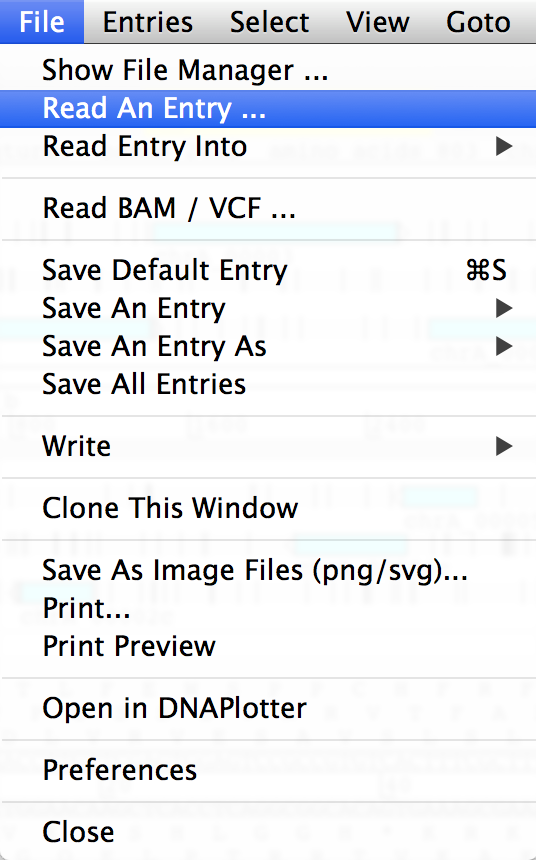
\includegraphics[width=0.3\textwidth]{images/artemis_cdspred0}     
    \end{center}
\end{frame}

\begin{frame}
  \frametitle{Comparing predictions in Artemis}
  \begin{center}
    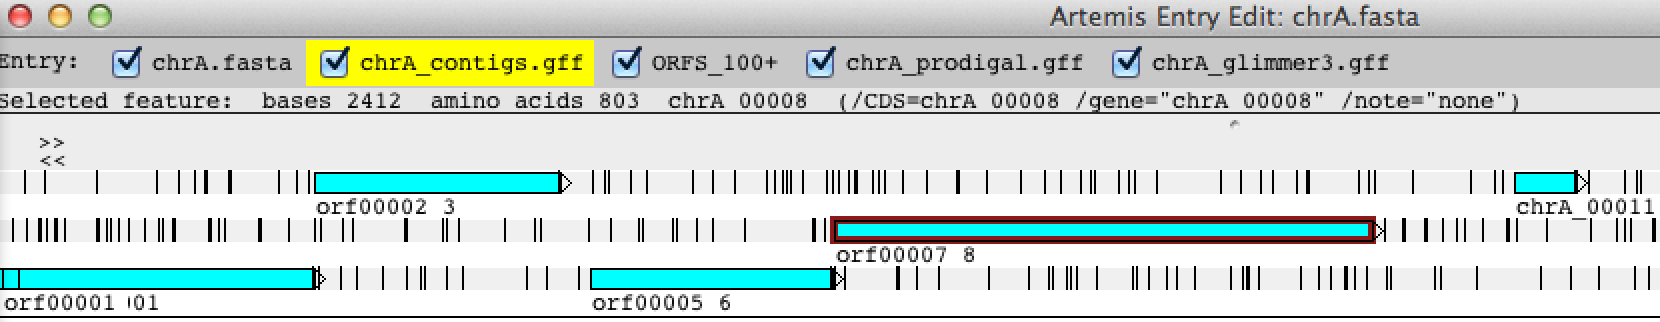
\includegraphics[width=0.9\textwidth]{images/artemis_cdspred1}     
  \end{center}
\end{frame}

\begin{frame}
  \frametitle{Comparing predictions in Artemis}
  \begin{center}
    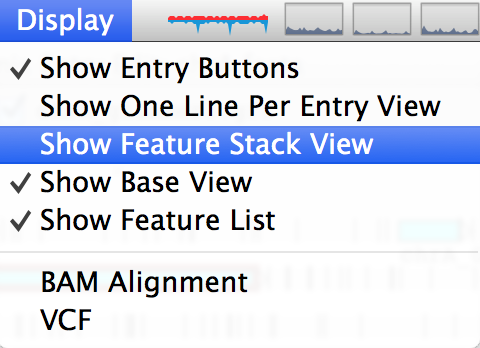
\includegraphics[width=0.4\textwidth]{images/artemis_cdspred2}     
  \end{center}
\end{frame}

\begin{frame}
  \frametitle{Comparing predictions in Artemis}
  %TODO - How to set the colours for each set of predictions?
  Do ORF(orange)/CDS(green,blue) prediction methods agree?
  \begin{center}
    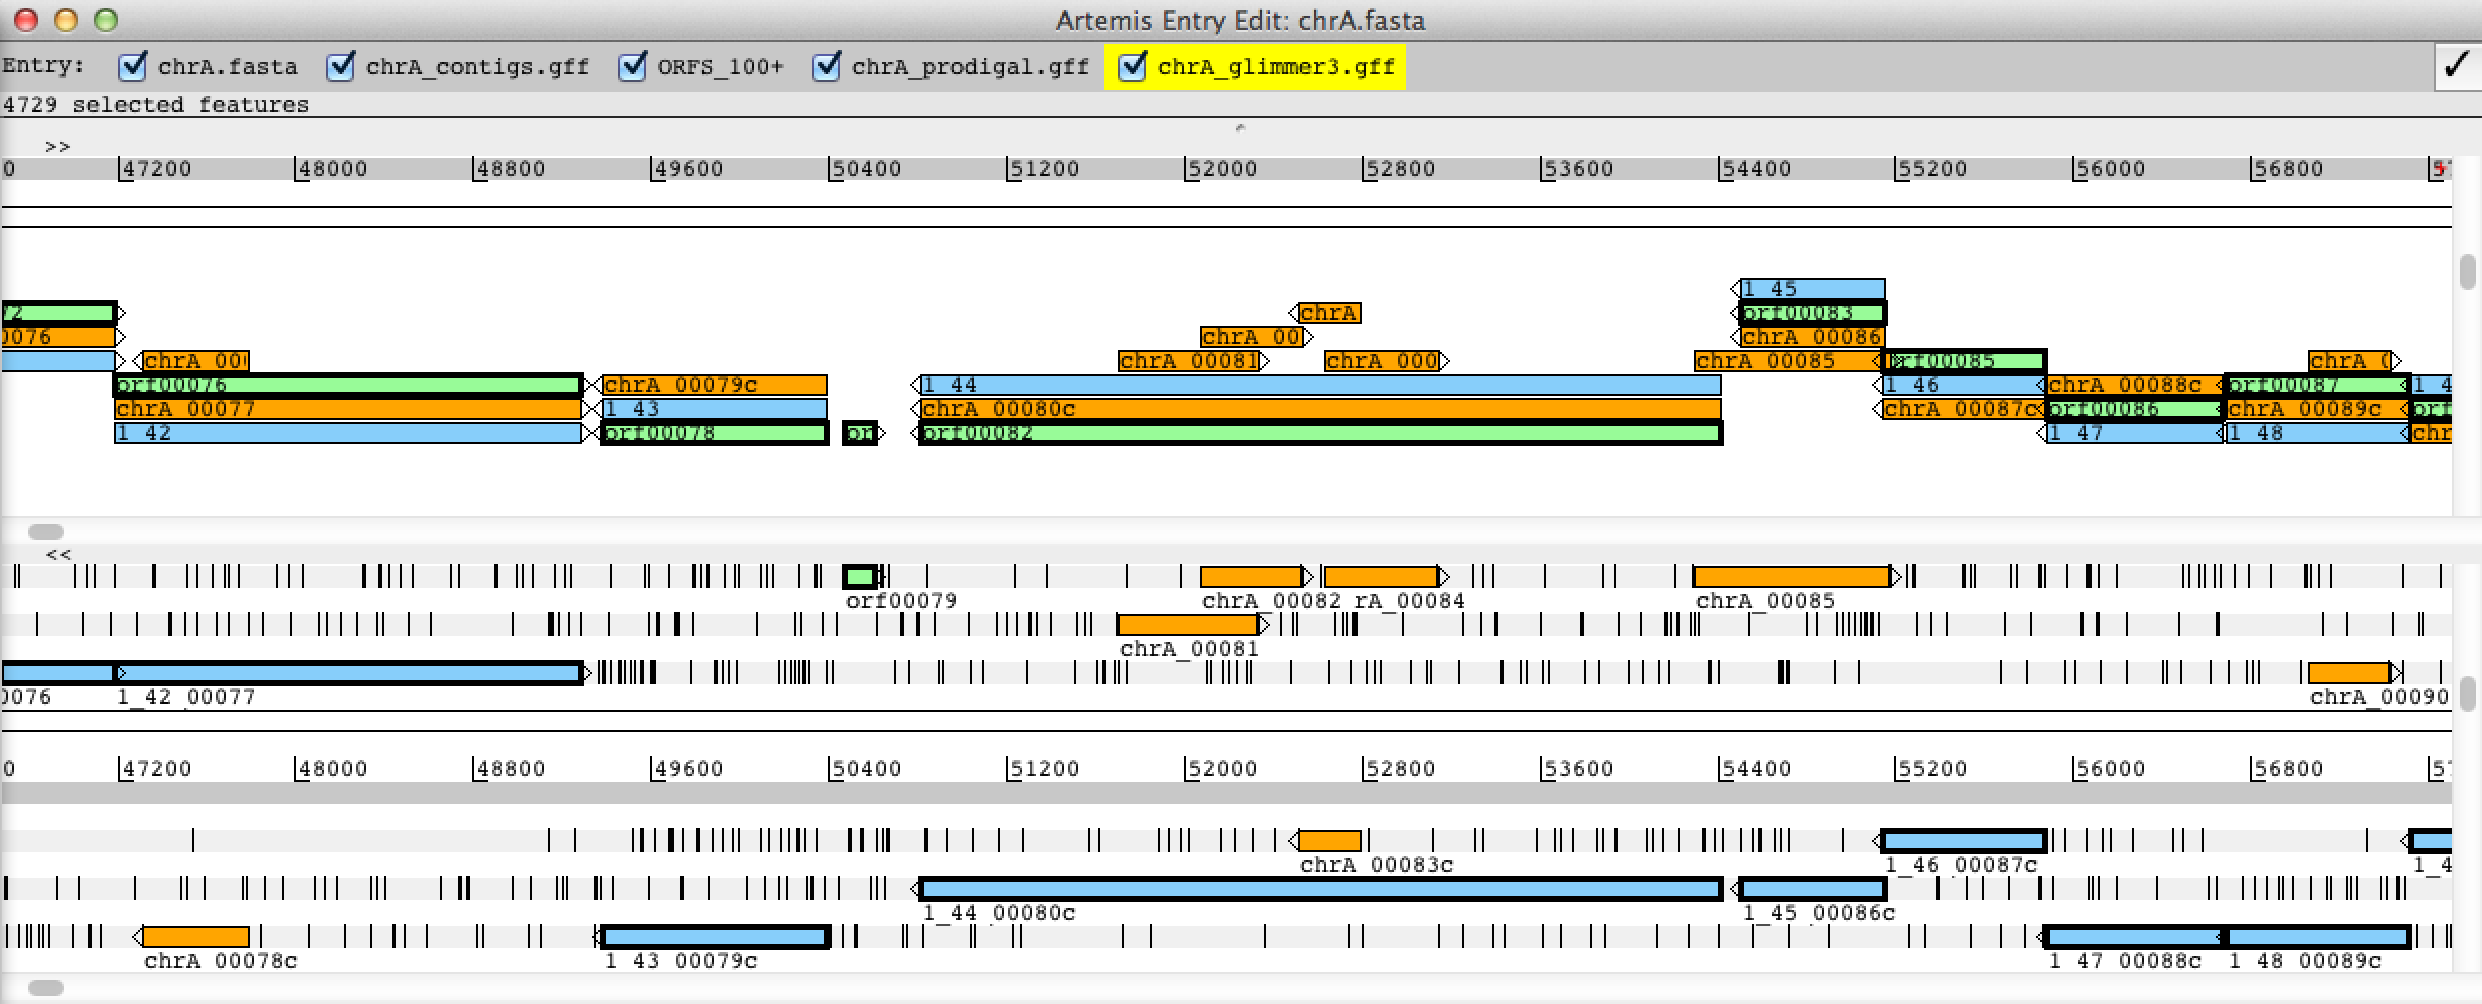
\includegraphics[width=0.9\textwidth]{images/artemis_cdspred3}     
  \end{center}
\end{frame}

\begin{frame}
  \frametitle{Comparing predictions in Artemis}
  Do \texttt{glimmer}(green)/\texttt{prodigal}(blue) CDS prediction methods agree?
  \begin{center}
    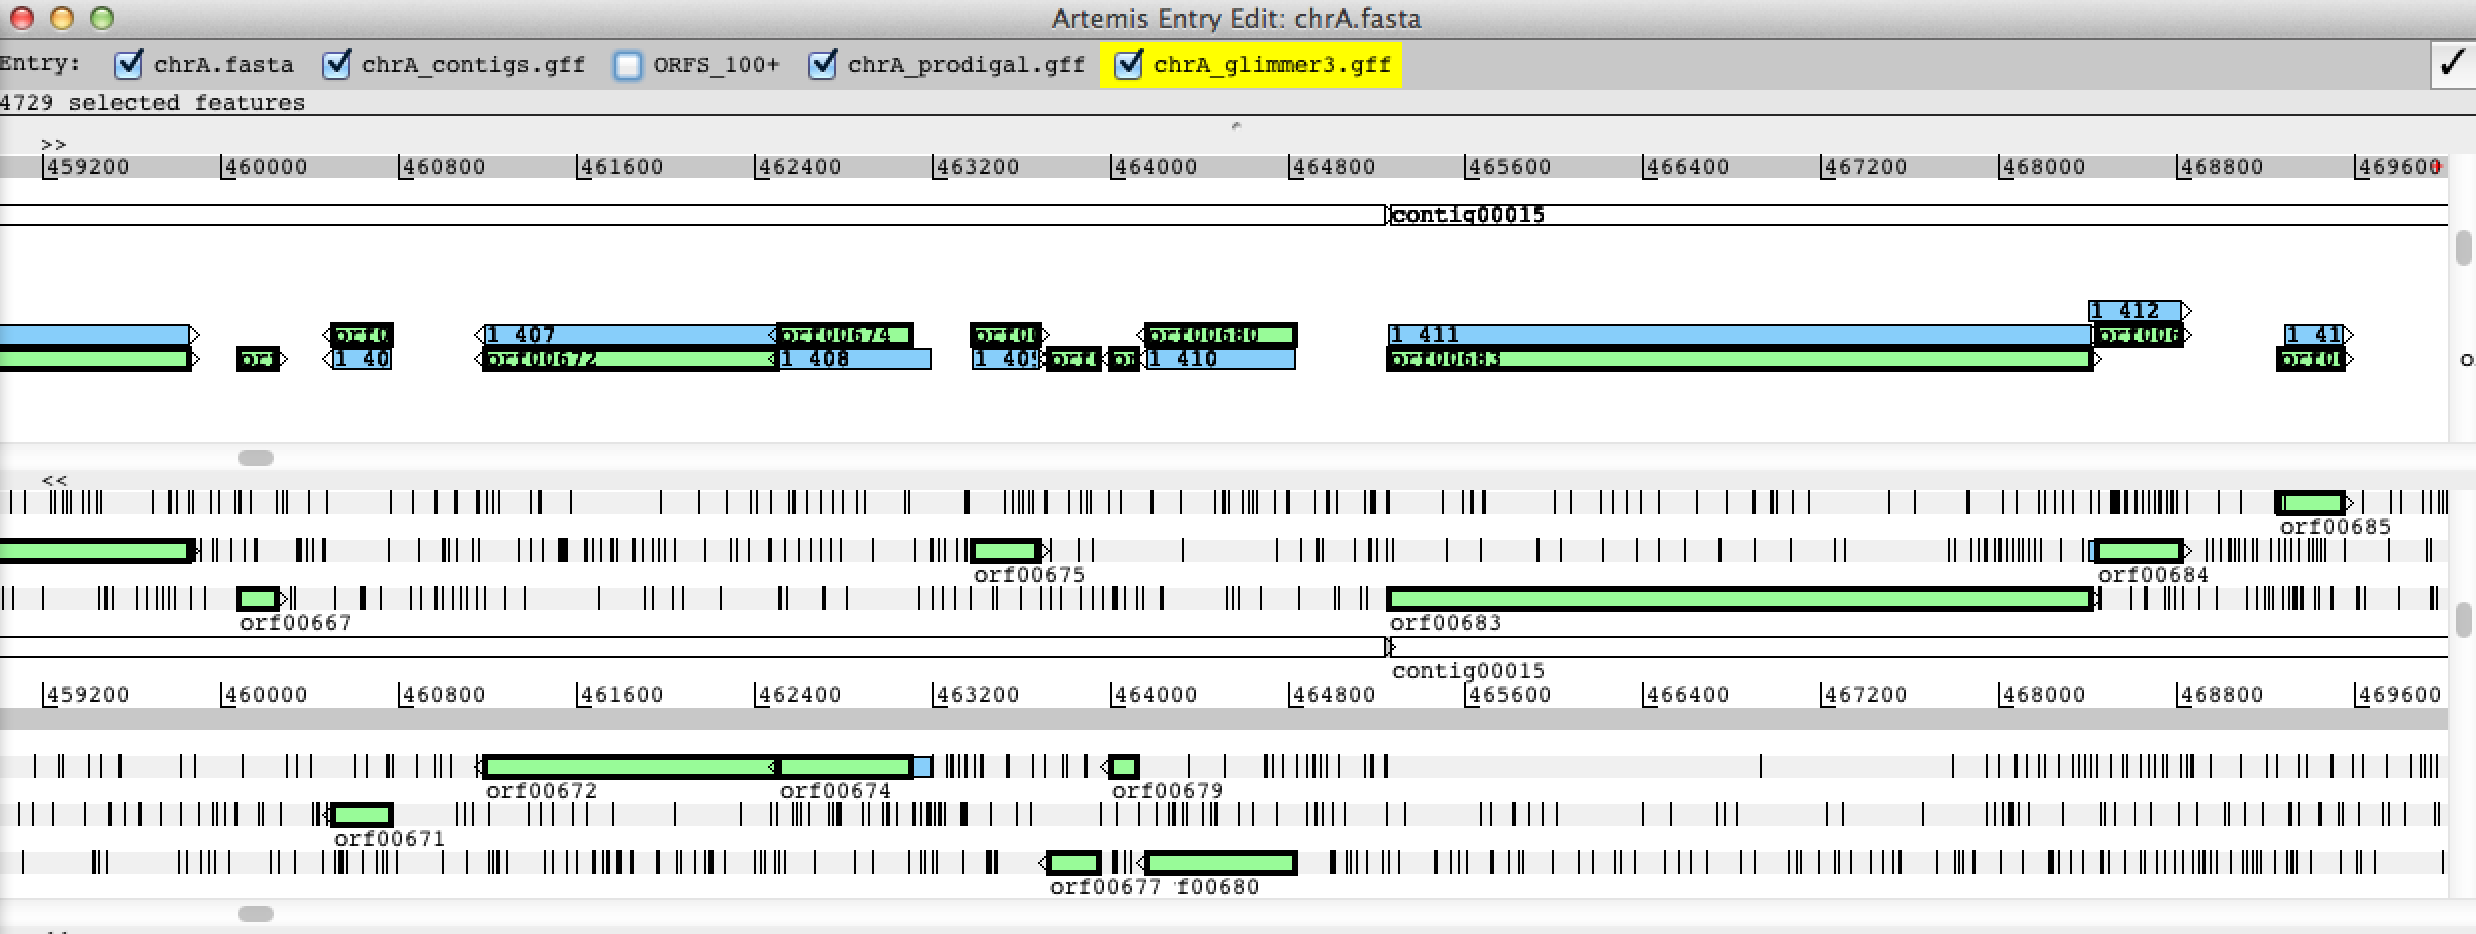
\includegraphics[width=0.9\textwidth]{images/artemis_cdspred4}     
  \end{center}
  How do we know which (if either) is best?
\end{frame}